% Options for packages loaded elsewhere
\PassOptionsToPackage{unicode}{hyperref}
\PassOptionsToPackage{hyphens}{url}
%
\documentclass[
]{article}
\usepackage{amsmath,amssymb}
\usepackage{lmodern}
\usepackage{iftex}
\usepackage{graphicx}

\ifPDFTeX
  \usepackage[T1]{fontenc}
  \usepackage[utf8]{inputenc}
  \usepackage{textcomp} % provide euro and other symbols
\else % if luatex or xetex
  \usepackage{unicode-math}
  \defaultfontfeatures{Scale=MatchLowercase}
  \defaultfontfeatures[\rmfamily]{Ligatures=TeX,Scale=1}
\fi
% Use upquote if available, for straight quotes in verbatim environments
\IfFileExists{upquote.sty}{\usepackage{upquote}}{}
\IfFileExists{microtype.sty}{% use microtype if available
  \usepackage[]{microtype}
  \UseMicrotypeSet[protrusion]{basicmath} % disable protrusion for tt fonts
}{}
\makeatletter
\@ifundefined{KOMAClassName}{% if non-KOMA class
  \IfFileExists{parskip.sty}{%
    \usepackage{parskip}
  }{% else
    \setlength{\parindent}{0pt}
    \setlength{\parskip}{6pt plus 2pt minus 1pt}}
}{% if KOMA class
  \KOMAoptions{parskip=half}}
\makeatother
\usepackage{xcolor}
\IfFileExists{xurl.sty}{\usepackage{xurl}}{} % add URL line breaks if available
\IfFileExists{bookmark.sty}{\usepackage{bookmark}}{\usepackage{hyperref}}
\hypersetup{
  pdftitle={arc42 Template},
  hidelinks,
  pdfcreator={LaTeX via pandoc}}
\urlstyle{same} % disable monospaced font for URLs
\usepackage{longtable,booktabs,array}
\usepackage{calc} % for calculating minipage widths
% Correct order of tables after \paragraph or \subparagraph
\usepackage{etoolbox}
\makeatletter
\patchcmd\longtable{\par}{\if@noskipsec\mbox{}\fi\par}{}{}
\makeatother
% Allow footnotes in longtable head/foot
\IfFileExists{footnotehyper.sty}{\usepackage{footnotehyper}}{\usepackage{footnote}}
\makesavenoteenv{longtable}
\usepackage{graphicx}
\makeatletter
\def\maxwidth{\ifdim\Gin@nat@width>\linewidth\linewidth\else\Gin@nat@width\fi}
\def\maxheight{\ifdim\Gin@nat@height>\textheight\textheight\else\Gin@nat@height\fi}
\makeatother
% Scale images if necessary, so that they will not overflow the page
% margins by default, and it is still possible to overwrite the defaults
% using explicit options in \includegraphics[width, height, ...]{}
\setkeys{Gin}{width=\maxwidth,height=\maxheight,keepaspectratio}
% Set default figure placement to htbp
\makeatletter
\def\fps@figure{htbp}
\makeatother
\setlength{\emergencystretch}{3em} % prevent overfull lines
\providecommand{\tightlist}{%
  \setlength{\itemsep}{0pt}\setlength{\parskip}{0pt}}
\setcounter{secnumdepth}{-\maxdimen} % remove section numbering
\ifLuaTeX
  \usepackage{selnolig}  % disable illegal ligatures
\fi

\title{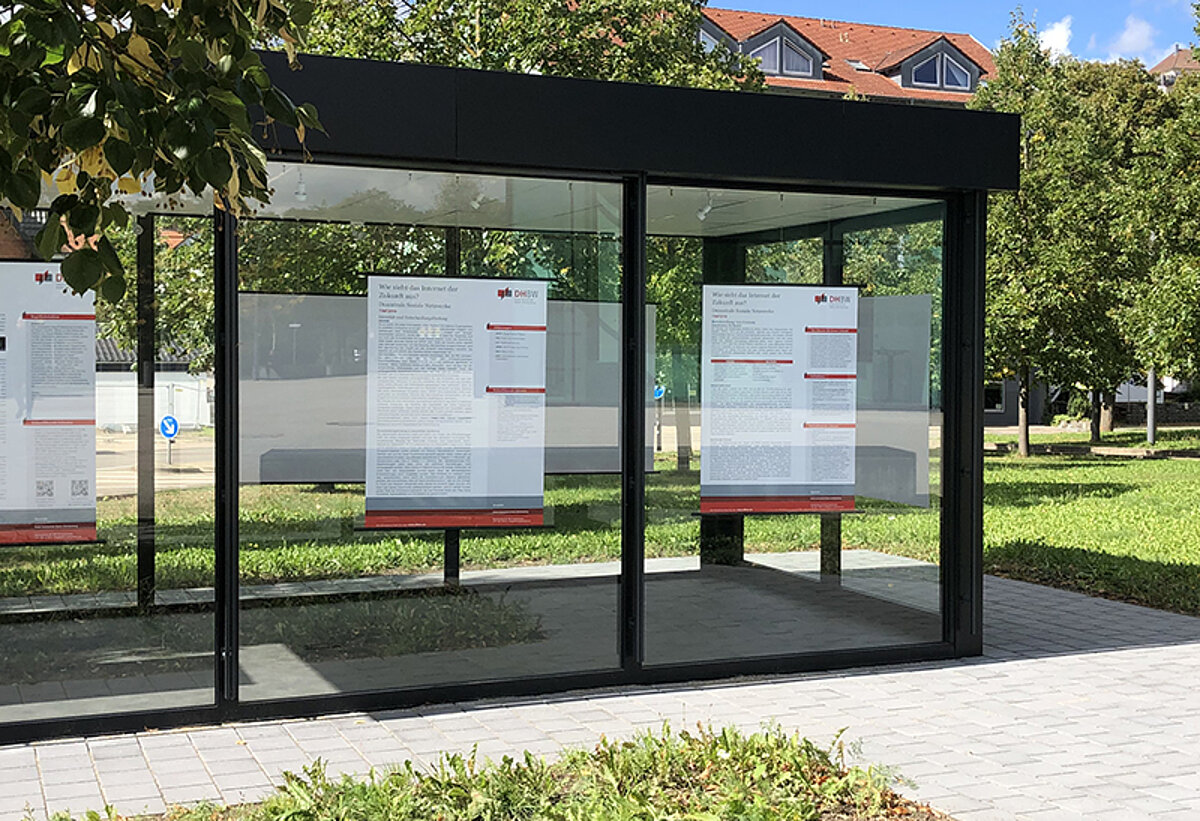
\includegraphics{header.jpg} Template}
\author{}
\date{Januar 2023}

\begin{document}
\maketitle

% DOCUMENT STARTS HERE


\hypertarget{section-introduction-and-goals}{%
\section{Einführung und Ziele}\label{section-introduction-and-goals}}

\hypertarget{_stakeholder}{%
\subsection{Stakeholder}\label{_stakeholder}}
Ein umfassender Überblick über die Stakeholder des Systems ist von entscheidender Bedeutung. Dies bezieht sich auf sämtliche Personen, Rollen oder Organisationen, die entweder die Architektur des Systems kennen sollten oder von dieser überzeugt werden müssen. Zu den Stakeholdern zählen auch jene, die aktiv mit der Architektur oder dem Code arbeiten, beispielsweise indem sie Schnittstellen nutzen. Ebenso gehören Personen dazu, die die Dokumentation der Architektur benötigen, um ihre eigene Arbeit effizient zu gestalten. Darüber hinaus sind Stakeholder involviert, die Entscheidungen über das System und dessen Entwicklung treffen.
Die nachfolgende Analyse zeigt alle Stakeholder gebündelt in ihren Gewichtungen und Beziehungen.  
\begin{figure}
  \centering
  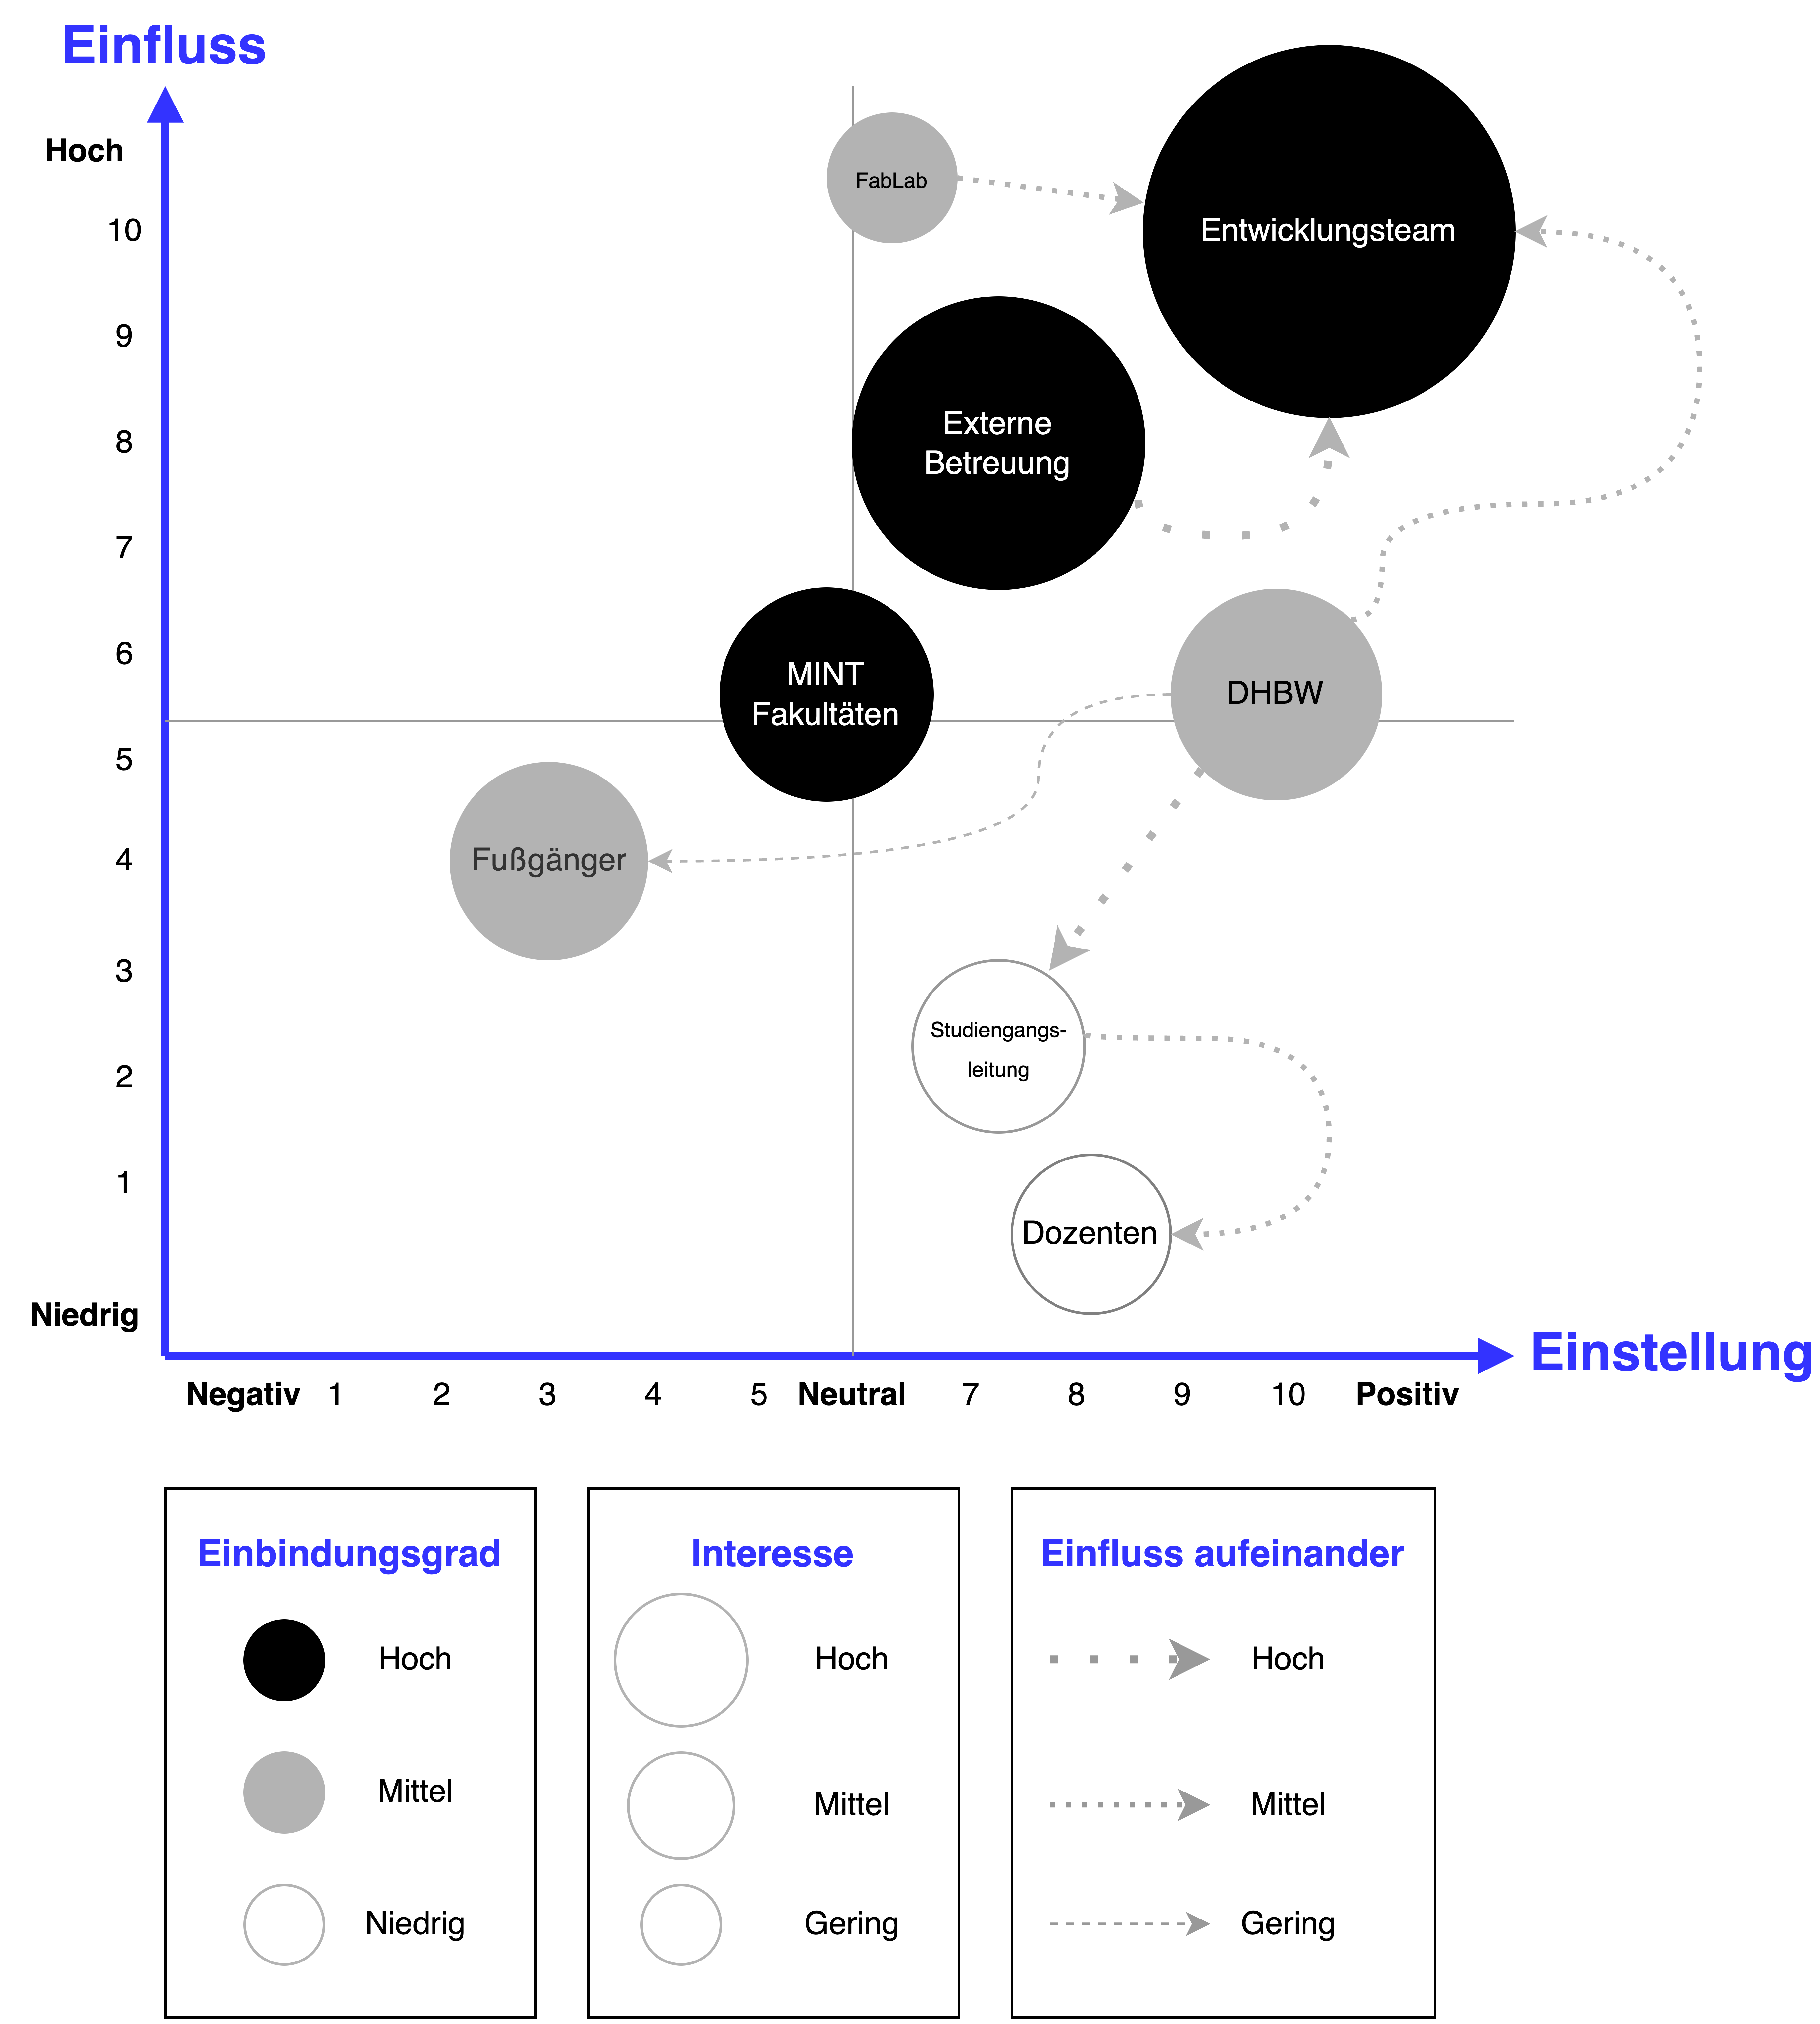
\includegraphics[width=1\textwidth]{./resources/stakeholderanalyse.drawio.png}
  \caption{Stakeholder Analyse und Zusammenfassung in den Unterscheidungen: Einbindungsgrad, Interesse und Einflüsse. Das Entwicklungsteam geht deutlich als am stärksten partizipativ gekennzeichneten Stakeholder hevor. Am repressivsten zeigen sich die Stakeholder in Form der Fußgänger.}
  \label{fig:deine_label}
\end{figure}

\section{Anforderungskonzept}
Die Anforderungen an die Umsetzung des Blickbox-Projekts werden in die Kategorien funktionale, nicht funktionale und hypothetische Anforderungen unterteilt.
Diese Differenzierung ermöglicht eine umfassende Abdeckung aller Aufgabenstellungen im
Zusammenhang mit der Umsetzung des Blickbox-Projekts.

\subsection{Funktionale Anforderungen (FA)}
  Funktionale Anforderungen beschreiben spezifisch die konkreten Zwecke, die das zu entwickelnde Produkt erfüllen soll.

\subsection{Nicht funktionale Anforderungen (NFA)}
Im Gegensatz zu funktionalen Anforderungen sind nicht-funktionale Anforderungen eher allgemein gehalten und betreen die gesamte Architektur und das Design des Produkts.
Sie können auf verschiedene Projekte angewendet werden.

\subsection{Hyptohetische Anforderungen (HFA)}
Hypothetische Anforderungen werden aufgrund von unsicheren Ergebnissen und vorherigen Abhängigkeiten definiert. Ihr Zweck besteht darin, mögliche Entscheidungen und Eventualitäten abzudecken, die eintreten können oder auch nicht.

\\
\\
\begin{center}
  \begin{tabular}{|p{\linewidth}|}
    \hline
    \textbf{Datenerfassung und -übertragung (FA1)} \\
    Beschreibung: Das IOT-System muss in der Lage sein, kontinuierlich Sensordaten zu erfassen.
    Diese Daten sollen im Raspberry PI gespeichert und verarbeitet werden.
    Die Datenübertragung auf den Server erfolgt Event-gesteuert und drahtlos.
    Die Daten werden nicht in Echtzeit, sondern in festgelegten Intervallen übertragen und festgehalten. \\ \\
    \hline
    \textbf{Bereitstellung eines Dashboard (FA2)} \\
    Beschreibung: Die Daten der Datenbank sollen mit Grafana grafisch dargestellt werden.\\ \\
    \hline
    \textbf{Interaktivität zu Dritten (FA3)} \\
    Beschreibung: Der Ausstellungscontainer soll attraktiver werden und Fußgänger sollen mit ihm interagieren können.
    Das soll in Form eines Displays oder Ton und Licht geschehen. \\ \\
    \hline
    \textbf{Präventive Lösung für Datenverlust (FA4)} \\
    Beschreibung: Ein default-Programm auf dem Raspberry Pi sichert, eine ungestörte Funktionalität der Ausstellungsbox.
    Die Daten puffern wir auf dem Pi, damit die Datenbank nur zur Darstellung in Grafana existiert.\\ \\
    \hline
    \textbf{Bereitstellung einer geeigneten Umgebung für die Hardware (FA3)} \\
    Beschreibung: Die Hardware soll sich im Ausstellungscontainer an einem trockenen, sicheren Platz befinden.\\ \\
    \hline
    \textbf{Containerisierung (FA6)} \\
    Beschreibung: Die Anwendungen sollen in Containern gekapselt werden. \\ \\
    \hline
  \end{tabular}
\end{center}

\begin{center}
  \begin{tabular}{|p{\linewidth}|}
    \hline
    \textbf{Erweiterbarkeit und Wartung (NF1)} \\
    Beschreibung: Die Architektur und Dokumentation soll möglichst zugänglich gehalten werden. \\
    Erweiterungen und Verbesserungen der Features sollen durch die Dokumentation und einen vereinfachten Hardwareaufbau erleichtert werden. \\ \\
    \hline
    \textbf{Sicherheit (NF2)} \\
    Beschreibung: Die Verbindung zum Server soll verschlüsselt sein. \\ \\
    \hline
  \end{tabular}
\end{center}

\end{document}
